\chapter{MONEY, BANKING AND CENTRAL BANKS}
\begin{chapquote}{Satoshi Nakamoto, Genesis Block}
``The Times 03/Jan/2009 Chancellor on brink of second bailout for banks.''
\end{chapquote}

\section{Banking and money}
The objective of a bank is to make profit by providing money belonging to people that don't need it immediately to people that instead need it for some purposes.

\subsection{M0, M1 and reserve ratio}
Imagine a world in which there are $N$ coins of gold owned by the people and one bank. These coins are not needed by the people, but there is a guy with a very good idea and wants to start a business that will help society, but he needs a fraction $f$ of $N$. If it's safer for people to store gold in the bank and if the business plan seems reasonable, then the bank will borrow gold from the people with an interest rate of $r_B$ and will lend it to the business man with a higher interest rate $r_L$. If the business succeeds, then the employees will get gold as a salary and they will store it again in the bank. At this point we know that there are still $N$ coins of gold physically, but in fact they are more. They are $N$ from the initial people and $fN$ from the employees. The former value is called \textit{M0}, the second value is called \textit{M1}. This works only if the business really succeeds in its work.

If a person comes to this bank and gives her gold in exchange for cash or a checking account, then she will be able to write checks for payments to other people. A checking account can be opened also for a person who needs a loan from the bank~\footnote{Remember, a loan in this case is an asset for the bank.}. Checking accounts are always liabilities for the bank.

The reserve ratio in this example is the ratio between the amount of gold in the bank and the quantity of gold corresponding to all the checking accounts and cash in the demand liabilities, which is also the ratio $M0/M1$. This ratio cannot be lower than a certain threshold. This percentage indicates what is the percentage of the clients that can come back to the bank and ask for their money at the same time. If more than that percentage suddenly show up, the bank won't be able to provide the liquidity. The smaller the reserve ratio, the better for the bank because it can make profit from all the investment, but as always this comes with risks. A banking system with a reserve ratio different from 1, is called fractional reserve banking

\subsection{Solvency, liquidity and leverage}
Solvency, or being solvent, is when the assets are larger than the demand liabilities―assuming the loans in the assets are good. This means that a bank can pay all the creditors within a certain amount of time. Insolvency happens usually when loans in the assets are not paid back and this results in negative equity for the bank. Keep in mind that a bank can have a checking account for someone, say a company, as a demand liability with a corresponding loan to the same company as an asset. If the company writes checks to other people, but then it's not able to pay back the loan, the bank must have money to pay the check to the people.

The leverage is the ratio between assets and equity. Assuming the bank has only demand liabilities $L$, then the leverage $l$ can be also written as: $l = \dfrac{A}{E} = \dfrac{L+E}{E} = 1 + \dfrac{L}{E}$. With a given leverage of $l$, a bank could bear a loss $pA$ if $pA < E = \dfrac{A}{l}$, which means the higher the leverage, the smaller the losses a bank can afford.
An alternative, but equivalent definition of leverage is the ratio between demand liabilities and equity $l = \dfrac{L}{E}$. 

In the real world there are multiple banks. If these banks have different reserve ratios, things might go wrong. What happens if the bank with the lowest reserve ratio becomes illiquid? People will stop trusting banks and a bank run will happen. It would be better if the bank with the highest reserve ratio lent money to the illiquid one, so as to avoid a bank run that would kill all the banks. 

\subsection{The central bank}
To avoid this problem of liquidity, there exists a central bank which combines this reserve of money. Each bank can have a different reserve ratio and when a bank need cash, more than its current reserve, it can get it from the central reserve. Furthermore, to make people feel more safe, this central bank is linked with the government. This means that the government can raise taxes or issue money and provide them to the creditors. 

In society there is sometimes the need to increase the money supply, for example when there are more people, or more factories and businesses producing wealth. To achieve this, the central bank prints bank notes and the government issues obligations. Citizens then buy obligations from the government hoping to make some money in the future. The central bank finally buys these obligations from the citizens\footnote{This is an open market operation, so the seller of the obligation does not know the buyer (the central bank, in this case).}, which can in turn put money back into their bank accounts. The net result is that there is now more money in the system.

In theory, a central bank has no equity and the liabilities it has with other banks have no interests. The assets are composed of cash and obligations (treasury bonds for example) that generate profit. In practice, a positive equity goes to the government and a negative equity means the government will provide money.

\subsection{Target rate}
If two banks have different reserve ratios and bank $A$ needs some cash for one day (overnight) from bank $B$ with higher reserve ratio, $A$ will ask for a loan and $B$ will give it a certain interest rate. The central bank, as already explained, can print money and then buy obligations from people than in turn will put their money into banks. This will result in banks having more money, so $A$ will need less money and will be willing to pay a lower interest rate and $B$ as well will be willing to offer a lower interest rate. The target rate (fed fund rate) is the rate at which the central bank wants other banks to lend money to each other\footnote{It is on an annual basis, then if money is needed for just one day, it is just a fraction of it.}. The central bank can increase it, as said before, but also decrease it by buying obligations (short-term treasury bonds that are less risky). The reason why they use this parameter to decide on monetary policy is that its value is easily accessible, just ask a bank for a loan. Instead, measuring the value of $M0$ or $M1$ is much more difficult and not real-time. 

The central bank tries to manage the target rate, which is the interest rate at which banks lend money to each other, but by increasing the money supply the cost of lending will decrease, so also companies and people will get cheaper loans.

Another reason why dealing with interest rates instead of amount of money available is that it allows to select businesses in a better way. What does this mean? Imagine we have 4 different companies, each with a project to finance and in need of the same amount of money $S$ but they are willing to pay different interest rates for their businesses: Good business plans will be willing to pay higher interest rates. If we focus on interest rates and we tune them depending on the period (growth or not), we can set a sort of threshold on how good a business should be or, in other words, how much wealth it should be able to generate. If we focus on available money instead we would always finance the best businesses and this is a problem in periods when there are no good projects to invest on. 

A repurchase agreement is when party $A$ gets a loan from party $B$ covered by some assets belonging to $A$ and also a repurchase agreement is given to $B$. This agreement says that $A$ will buy back its assets from $B$ but at a higher price (the loan + interests).

\subsection{The discount rate}
When a bank has no more liquidity and it's not able to get loans from other banks at the fed funds rate (target) because they don't trust it, then it's last option is to ask for a loan to the federal reserve but with a higher rate, the discount rate. The money from the central bank is printed, not taken from the previous assets.

When a person puts money in the bank, she can be told she can withdraw the money at any time or that she can withdraw only 10\% of the money at any time and the rest later. In the second case, one should ask for interests because the bank is using her money to make profit.

\subsection{Federal Deposit Insurance Corporation}
With fractional reserve banking, one bad bank (with money invested in bad loans) may lead to big problems for every other bank. Moreover, A central bank can help banks in this situation, but it must be able to differentiate which bank is good and which cannot pay its debt (insolvent). In case the central bank is not willing to lend money to a bad bank, there is a second option. It's called Federal Deposit Insurance Corporation. The idea is that each bank pays a small percentage to the FDIC, a sort of insurance that in case of a bank has lack of liquidity, has made bad investments or is going bankrupt, the FDIC provides liquidity to the banks avoiding bank run. This percentage is usually lower than the interest rate of the loans provided to the people, so a bank is willing to use this insurance to be safer and also to lower interest rates to its clients. When there is a good period for the economy, the percentage paid to the FDIC is low, but when things go bad, it increases. It's interesting to note that this insurance does not have the same properties of normal insurances. Here, a bad event is usually correlated to other bad events because the financial system is connected. Instead, car accidents are usually uncorrelated and they spread throughout the time. A high interest rate is always seen as a risky investment, but if backed by the FDIC, it is much more secure. If a bank is insured by the FDIC, it is encouraged to make riskier investments, offering higher interest rates. 

\subsection{You don't need a fancy MBA}
Venture capitalists, private equity and hedge funds provide basically the same service of banks: get money from people who do not now how to invest and use it to finance some businesses. The big difference is that they do not operate on fractional reserve banking. They may say upfront that some part of the money is locked up for some years and some part is on demand (liquid), but there is absolutely no problem like bank run. Moreover, they add value to society investing in businesses and startups. Now the critic part. With fractional reserve banking a bank takes money from a normal person claiming that her money is always available―as long as a fraction of the population does not withdraw all their money. Since it's money almost "always available", she does not get a high interest on that money, but, by being insured by the FDIC, the bank can invest on much more risky companies with much higher interest rates or on long-term treasury bonds and make more profit\footnote{Sal's critic: "Anyone can do this. You don't need a fancy MBA to figure this out. This doesn't add any true value to society."}. All of this because of the FDIC. Note that when the FDIC has no more money, the government raises taxes on citizens. Is this even capitalism? Where is the competition? Where is the innovation? The most successful banks will have riskier investments and if everything goes wrong, there is the FDIC to cover the losses\footnote{"The banks are holding us at gun point and threatening to take us all down with them if we don't bail them out. They argue that if they go down the economy tanks with them since there will be nobody to give out loans when they're gone. Unfortunately, this is true to an extent because the government allowed them all to consolidate to the point that if a single one of these big banks failed there would be enough paperwork to send the economy to a screeching halt." Comment from FishHead}\footnote{"What the FDIC's intervention leads to though, is to reduce the risk to depositors to 0 (by taking onto itself any catastrophic loss, like what happened in the mortgage crisis). The fact that the depositors have 0 risk to their money means that they accept to give it to the bank to very low interest rate (like Bank of America that was (and might still be, not sure) giving 0.1\% interest rate on the money to depositors). If there was a risk to give money to the bank, because it was not FDIC insured, the only way people would put it there is if there was a decent amount of interest accumulating." Comment by Patccmoi}.

Another useful parameter is the LIBOR, London Inter-bank Offered Rate, an average rate at which banks lend money between themselves.

\section{Quantitative easing}

So far, we know that the central bank can buy short-term treasury bonds to lower the fed fund rate (target). This is injecting money to the system and lowering the yield curve where the maturity time is short (few days). By keep buying bonds, this rate can reach zero. What if this is not enough to stimulate the economy? The central bank can start buying long-term bonds, lowering again the yield curve. It can also buy mortgage-backed loans, or corporate debt to make the market more liquid. This is quantitative easing. 

In quantitative easing generally, the central bank is trying to lower the yield curve, first with treasury bonds. The hope is that by doing this, also other rates get lower, such as mortgage loans and corporate debt. If this does not happen, it is dangerous because the spread (difference) between treasury bonds and other types of debt increases. In 2009 Bernanke tried to avoid this danger by buying exactly these assets to increase demand and lower interest rates in these specific markets and he called this "credit easing". Japan instead did quantitative easing just for the sake of printing money without paying much attention on where the money was going.

\section{2008 bank bailout}

\subsection{Mark-to-model or mark-to-market writedown}
As already seen in section \ref{Corporate metrics and valuation}, a company provides a book value for its equity, based on its analysis of assets and liabilities. This may differ from the value of the market. This happens usually because the value of some assets are valued differently by the company and the market. If the book value and the market value differ a lot, the company can do two things: mark-to-model or mark-to-market writedown. In the first case, the company asks some special analysts to create fancy models and valuate their critical assets (mostly derivatives and other toxic assets) leading to a correction, or writedown, of their total assets' value. In the second case, the company simply looks at the price of those critical assets in the open market. In the former case, the assets value may be biased in favor of the company, in the latter it may be biased against the company and in favor of the skeptics because in the open market people sell and buy driven by their feelings (fear, excitement).

\subsection{Bank bailout example}
A typical scenario of bank bailout is the following. A bank has assets like cash, treasury bonds, AAA corporate bonds, and derivatives and has liabilities such as loans to different entities. Usually this loans are interest-only meaning that during the loan only the interest gets paid while the loan is paid at once at the end\footnote{This is done to take advantage of tax-deductible income as already seen in section \ref{mortgages} and \ref{Personal taxes}.} and what happens is that the loan will be renewed at its expiry date and it remains interest-only. The problem arises when the lender of the loan does not want to renew it because for example the debtor owns toxic assets (assets that are worthless or difficult to sell). Now the debtor―the bank in our case―has to pay back the entire loan and to do get money immediately it starts selling treasury bonds. The same process repeats when other loans mature and if the bank does not have any more treasury bonds, then it can sell AAA corporate bonds, which are still easy to sell, but probably not at the expected price, so the equity starts shrinking. The critical step is reached when the bank has to pay back a loan but the only remaining assets are cash and toxic derivatives or the like. Here, the bank cannot use cash because they need it for the daily operations, so it tries to sell the derivatives, but they have to be sold at price $X$ such that it allows the bank to pay back all the debt it has, otherwise it would be useless and the bank would go bankrupt anyway. If the market is not willing to buy these assets at price $X$, then there are two choices―at least.

One option for the bank is to issue shares and find an investor―usually a foreign entity with the currency used by the bank or a sovereign wealth fund―willing to buy them such that the bank can then pay back the last loan or loans. Of course, the losers here are the shareholders because the equity decreased a lot and new investors join. At this point, the bank is left with some cash, toxic assets\footnote{The bank hopes they will become good investments in the future.}, no liabilities and equity, so the bank is de-leveraged and it has been bailed out.

A second option is bankruptcy (see section \ref{Life of a company}). Here the company can completely shut down after the liquidation of all its assets or can still operate but the previous shareholders are wiped out and the last creditor of the company becomes the new single shareholder with new shares and only liquid assets (toxic ones are sold, regardless of their value).

\subsection{The moral hazard and the incentive to create bubbles}
Imagine a scenario in which a lot of banks have toxic derivatives as assets or CDOs (Collateralized Debt Obligations) and they owe money to each other in form of loans. If one bank discovers that its toxic assets are worth less than the equity, as in the case seen above, then this bank becomes insolvent and this lead to a chain reaction in the whole banking system. If a creditor bank now loses money because of this insolvent bank, on top of its other risky investments, it too will face difficulties or bankruptcy. More generally the problem is not related to only one risky asset, rather all of them deteriorate and are worth less.

To avoid this problem, the central bank can decide to buy more risky derivatives and CDOs from the banks, hoping that this money will enter the system and start circulating, but also to create demand for these assets with a reverse auction\footnote{In this case, a reverse auction means that the central bank is willing to buy toxic assets from the lowest (cheaper) bidder.}\footnote{Sal is skeptical about this point. If there were people willing to buy these toxic assets, they would have already bought them, without waiting for an artificial demand created by the central bank. Also, if a bank is selling these toxic assets all the other banks will stay away from this bank because they know its a risky bank}. In 2008 though, this did not quite happen because banks were so afraid (their toxic assets were worthless and that they weren't able to pay back their loans) that they did not spend this money, holding it tight for loans due in the future.

When the central bank buys these toxic assets, it should not buy them at fire-sale price (the price of a panicked marked, so extremely discounted prices), but rather at a price that allows the banks to keep a non-negative equity. By doing this, though, the central bank is literally writing a check to the shareholders and to the creditors of the banks at risk, the very people to blame for the problem. The counterargument is that if the central bank does not follow this path, the entire economy will collapse. So hoping that banks fail and go bankrupt may be a good punishment for the bad investments and misbehavior of the bankers, but on the other side there are real businesses and companies that will lose their money because of this event and all the system, not only the banking one, will suffer. 
The deeper problem, or moral hazard, is that when times are good bankers gets a lot of money, bonuses and so on, but when times are bad they can rely on the government and the central bank to cover the losses. This is definitely an incentive to keep creating bubbles and keep taking huge risks.

As explained above, the central bank can print money and buy toxic assets from a bank, but it can also decide to buy new stocks from the bank so that the current share holders are no longer the majority and the bank can pay its debt. By doing so, though, the central bank is helping the bad investors which lent money to the bank. If the central bank is really worried about the real economy and does not care about saving banks because they will come back anyway in few years―hopefully more conscious and with proper risk measures―it should create a fund that will pay back the loans to businesses and people that would have otherwise lost their money they kept in the banks.

\subsection{Worthless CDOs}
But how is it possible that CDOs are worth nothing? Let's see an example. Assume there is a special-purpose entity which lends money in form of mortgage loans, say $N$ loans, to people for a total sum $S$. Of course, to lend money this entity must raise money first. To do this, it splits the sum $S$ into $n$ tranches so that the first one has an interest rate $r_1$, the second one has an interest rate $r_2$ and so on until $r_n$, with $r_1 < r_2 < ... < r_n$, meaning that the first tranche is the least profitable, but it has the highest seniority\footnote{It will be paid first in case of bankruptcy} and the last one is the most profitable, but very risky. Now, even if one single mortgage loan is not paid back to this special-purpose entity, there will be at least one investor that will lose money. The higher the number of unpaid loans, the higher the number of investors that will lose money.

\subsection{Merrill Lynch and the Loan Star Funds' affiliate}
At the end of June 2008, Merrill Lynch had to write down some of its assets from \$30.6 billion to \$11.1 billion. These assets were super senior ABS (Assets-Backed Securities) CDOs. On July 28th, Merrill Lynch agreed to sell these CDOs to an affiliate of Lone Star Funds, a private equity, at a price of \$6.7 billion. This affiliate was financed for this investment by Merrill Lynch itself for 75\% of the total amount, meaning that the affiliate―financed by Lone Star Funds―put \$1.7 billion and got \$5 billion as a loan. In case of insolvency, both parties agreed that the affiliate will not lose more than \$1.7 billion. Say that three months after July, the value set by the market was \$10 billion, then of course Lone Star would profit by \$3.3 billion by selling, and Merrill Lynch could get back their \$5 Billion loan. The fact is that this scenario was quite unlikely to happen, but Merrill Lynch was able to artificially create demand for the CDOs and avoid writing them down immediately and the affiliate was able to get the CDOs paying 6\% of their original value (\$1.7B instead of \$30B).

\section{Geithner plan}
To save the banks in the financial crisis in 2008, the federal reserve came up with a plan where private investors and the central bank team up to create a unique entity. In this entity, the private investors―expert traders that know how to value stocks and bonds―are the shareholders together with the treasury. The private investors contribute a small percentage to the initial assets and the rest is financed with a loan by the fed. The purpose of this entity is to fix a price for the toxic assets of the banks and buy them. If these assets turn out to be non-toxic then the private investors will make money and the loan will be paid back to the fed. If instead these assets are worthless, then the private investors will lose a small amount of money, while the fed will lose more (a fraction of or the whole loan). 

It is interesting to note that nothing can seriously prevent the bank itself to be the private investor in this new entity. This can lead to an overprice of the toxic asset and the bank will face much smaller losses. A possible scenario is the following. The bank with toxic assets starts selling CDSs on those assets with very low interest rates, which means a very cheap insurance on a bank's default. Then, a hedge fund or, more likely, the shareholders of the bank with toxic assets will buy these cheap CDOs to edge their losses in case these assets turn out to be worthless, but they also put money into the special entity with the central bank to save the banks. Now, in case these toxic assets turn out to be good assets, the hedge fund makes money because it has a share in this entity, but in the opposite scenario thanks to the CDSs they don't lose money.

As explained so far, this plan is very much like a put option of the toxic asset. Let's see. Assume that the initial value of this toxic stock was $I$ and the hedge fund was ready to invest the same amount of money on the stock, but it had two possible alternatives, joining the Geithner plan or the put option plus the stock. In the first case, assume the hedge fund is investing a sum $S$ in this special entity, with $S = r \cdot I$ and $r = 15\%$, meaning that $I-S$ is put aside. The Treasury will match this sum and the entity will have an equity $E = 2S$. The central bank then puts a sum of money $L$, so that the banks are able to cover their debt and the entity is capitalized with a total sum $T$. Let's also assume this special entity now buys $N$ stocks for a total price of exactly $T = N \cdot I$. Now, if the stock value in the future $V$ will be such that $NV \leq L$, the hedge fund and the treasury make no profit, but the hedge fund remains with the initial sum $I-S$ that it put aside. If the stock value will be such that $NV > L$, the hedge fund's profit is $P = \dfrac{NV - L}{2}$ but it also has the initial sum $I-S$ that it put aside. The equivalence is shown in Figure \ref{fig:GPlan_HF}.
\begin{figure}[h!]
\centering
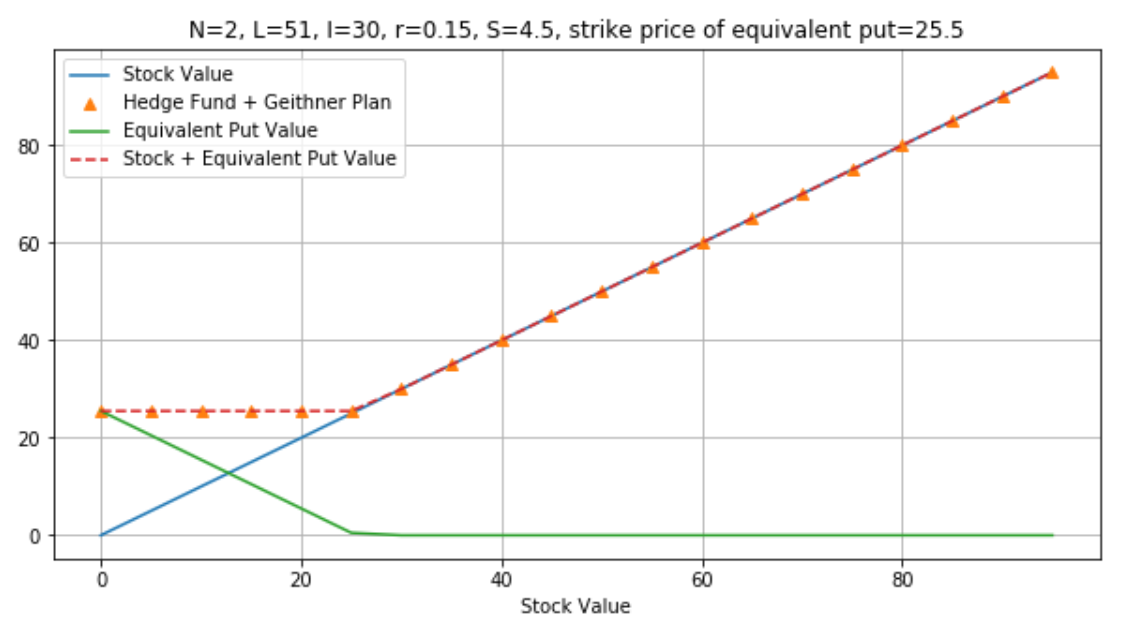
\includegraphics[width=0.8\textwidth]{images/GPlan_HF.png}
\caption{Comparison of the value diagram for a put+stock and the possible Geithner plan exploit.}
\label{fig:GPlan_HF}
\end{figure}
That being said, we can conclude that, to a rational investor, joining the Geithner plan or buying a stock and the put option is equivalent. The second scenario means that the investor should buy the stock at a value $I$ and the put option at a certain price $p$ (which can be computed using the Black-Scholes formula). With the numbers presented in Figure \ref{fig:GPlan_HF}, a reasonable value would be $p = 20$. This means that the investor is willing to put at most $50$ to join the plan. The problem is that this sum from the private investors was not enough to cover the debt of the banks. The banks themselves could form other entities to join the plan as already mentioned.

A possible solution proposed by Sal is that the toxic assets are put into another new company with toxic assets only and then it starts selling shares to the open market (e.g., NYSE). This new company should be transparent, explaining what are the assets so that any investor can easily decide whether to buy or not. Otherwise these assets would remain obscure and hard to buy for the majority of the investors, reducing the demand and decreasing their price. If the new shares are worthless, then the bank will fail, but at least it will happen in a transparent way and probably with lower likelihood.

\section{Foreign exchange and trade}
Imagine a simplified scenario where there are 2 people, Alice and Bob, willing to exchange RMB with USD and one person, Chen, willing to do the opposite exchange. Both Alice and Bob have 100 RMB and Chen has 100 USD only. Chen decides to put part of his money to the open market to be exchanged in USD. As soon as Alice notices it, she accepts to exchange all her RMB into USD at the rate proposed by Chen: $1 RMB = 1 USD$. Chen understands that there is quite a lot of demand for the currency he has, given that Alice accepted immediately, so he decides to change the rate for the remaining part of his currency: $1 RMB = 2 USD$. Bob has still his 100 RMB and given the fact that last time he wasn't able to exchange the sum because Alice was faster, now accepts the new and worse rate proposed by Chen. In this scenario, the price of USD went down compared to RMB and the price of RMB went up compared to USD, meaning that it is now a bit more difficult to buy RMB with USD (you need more USD to get one RMB) and it is easier to get USD with RMB (you need less RMB to get one USD). Notice that there is no relationship between the fact that the price of RMB as gone up compared to USD and the ratio between the amount of RMB available and the amount of USD available. It all depends on the offer and the demand.

Imagine now that Chen needs to sell $n$ units of his product at $X$ RMB each in the USA, where Alice lives, in order to cover the costs and make some profit. Alice instead needs to sell $m$ units of her product at $Y$ USD each in China, where Chen lives. If now they have to exchange their currencies with a rate $1 RMB = 1 USD$, Alice gets 100 USD and Chen gets 100 RMB. What if the next year, there is also Bob involved in the market? As seen above, Chen will change the exchange rate to $1 RMB = 2 USD$. This means that Chen will now sell his product in the USA for double of the previous USD price (but at the same RMB price if it would be in China), while Alice will sell in China for half of the RMB price (but at the same USD price if it would be in the USA). Doubling the price leads roughly to half of the units of product sold and vice versa with halving the price. This results in a balance between how much wealth (number of products times value of each product) is shipped in the USA and how much is shipped to China.

The main takeaway is that when there is more demand for currency A than its supply, its "price" compared to currency B will go up (more people want to have A but they have B). From a trade perspective this means that people from the country with B as currency can lower prices of products sold in the country with A, and vice versa, people from country with A and selling in the country with B should increase the prices, which will reduce the number of products sold. The trade imbalance will also decrease, eventually becoming balanced.

Assume we have an exchange rate $e = .87EUR/GBP$, this means that if we have 100EUR and we want to know the value in GBP we multiply 100EUR by .87 and we get 87GBP, simple. In general, with an exchange rate $e = r*A/B$, to go from a sum in A to a sum in B we multiply the sum in A by $r$. 

If $r$ decreases, A is getting weaker compared to B and it will be more expensive for people with currency A to buy products sold in currency B, which means more coins of A are needed to get one coin of B. This is bad for the consumers, but maybe not so bad from a trade balance point of view, because the country with A will be able to sell their products at lower prices in other countries.

If instead $r$ increases, A is getting stronger compared to B and it will be cheaper for people with currency A to buy products sold in currency B. This is good for the consumers, but maybe not so good from a trade balance point of view, because foreign countries will be able to sell their products at lower prices in the country with a stronger currency.

\subsection{Carry trade}
A carry trade is a situation where a currency A can be borrowed at interest rate $r_A$ and a currency B can be borrowed at $r_B > r_A$ with an exchange rate of $1 A = c B$, and this holds for a long period during which an investor can borrow a sum $S_A$ of A, convert it into a sum $S_B = S_A \cdot c$ of B, lend $S_B$, get $S_B' = S_B \cdot r_B$ in interest and convert back to A to get $S_A' = \dfrac{S_B'}{c} = \dfrac{S_B \cdot r_B}{c} = \dfrac{S_A \cdot c \cdot r_B}{c} = S_A \cdot r_B > S_A \cdot r_A$, making a profit of $P = S_A(r_B-r_A)$. This is free money, but as soon as people will spot this opportunity, we should have $r_A$ and $r_B$ converging to the same value.

\section{Chinese currency and U.S. debt}

\subsection{Pegging the yuan}
What the Chinese government and the Chinese central bank did was to keep printing yuan and trying to convert it into dollar to keep the exchange rate fixed, or pegged (e.g., $10 RMB = 1 USD$) so that for Americans it was always cheap to buy Chinese products. Printing yuan of course means depreciating its value, but on the other side, China was able to produce, sell and grow thanks to Americans buying their products. Chinese inflation is slowed down by a corresponding Chinese growth\footnote{We give China pieces of paper, they give us stuff we want. Does that sound like such a bad deal? - Andrew M.}. At the same time though, the American industries produce much less. 

Once the yuan is printed, the Chinese exchanges it with the dollar in the market. This big sum of dollars in cash are then used to buy safe and liquid assets: US treasury bonds. This leads to lower interest rates as there are more clients willing to get the bond and lower borrowing costs for the government, which means the government could lower taxes or spend more. Note that a central bank (the federal reserve in this case) can regulate only short-term interest rates and not long-term bonds. The net result is more cash in the American pockets, but it's not debt-free cash, it is financed by Chinese yuan.

By printing yuan, China can have an export-led growth and sooner or later, the Chinese will be able to buy products previously inaccessible to them, e.g., manufacturing products (washing machines) and the Americans will lose some low-price markets but will be able to focus on knowledge-based markets and have lower prices. As soon as the Chinese central bank stops printing yuan, the borrowing cost of a loan in USD will be higher and the exchange rate will change so that the prices will not be so low as before.

The Chinese central bank can also decide to buy other assets other than US treasuries, like UK bonds. This will make the GBP worth less compared to USD and to avoid this GBP appreciation, the British central bank would print GBP and buy US treasuries.

Just to give some real numbers, from November 2009 to November 2010, the Chinese central bank reports that the M1 value increased by roughly \$700 billion and around \$422 billion are used in foreign assets. This is again to keep the yuan cheap outside China.

What if the PBOC (People's Bank Of China) stops printing yuan? The yuan will become more expensive, stronger and less Chinese goods will be sold outside China, inflation will decrease and economy will slow down. India or other countries with cheap labor may take the lead in manufacturing sectors. The trade imbalance between China and other countries will decrease. The the interest rates in the US will increase as there is less demand of US bonds. Chinese imports to the US will become more expensive.

\section{2011-2012 Greek debt crisis}

\subsection{The problem}
From 2003 to 2012, the debt-to-GDP ratio of Greece went from 97.4\% to 198.2\% meaning that the Greek debt became twice as much as what the country was able to produce. From 2007 to 2012, the taxes payed by the Greek population were around 40\% of the GDP, while the public expenditures where around 50\% of the GDP, clearly not a good sign for their debt. This led also to higher interest rates for the Greek bonds as people started being suspicious about the Greek government's ability to pay back the debts. 

\subsection{No obvious solution}
One first thought might be to reduce the expenditures and increase taxes, but obviously this is not something a politician would easily do as he would lose consensus. The additional problem was that the GDP growth was negative during that period meaning that the country was in recession and implementing measures of austerity while recession is not a good move because it will slow down the economy, public revenues (taxes) will decrease and interest rates will increase. The solution here is not obvious, but what happened was that Greece received financial help from the EU and implemented at the same time austerity measures, but it did not lead immediately to economic improvements.

A bad idea would be to simply default on the debt. In this case the Greek government would not pay back the investors, but by doing so, all the investors will stop lending money and the state will not have money for pensions for example. It would be a drastic shut down of the government. This is not a good solution.

Being Greece part of the Euro-zone, the debt it was obtaining was pretty cheap thanks to the euro. Another hypothetical alternative, if Greece was not part of the Euro-zone, was to print more drachma, buy government bonds to finance the economy, increase inflation which might help to exit the recession. What's interesting in this possible solution is the following. Imagine Greece had a GDP of $\delta\rho$100B, obligations for $\delta\rho$10B, and a total debt of $\delta\rho$150B. Then in few years, the prices of the goods double thanks to the printed drachma by the Greek central bank. If the number goods and services produced in this period remain constant, but their prices double, the GDP (not adjusted to inflation) will be $\delta\rho$200B, while the obligations and the debt will not change. This is of course something bad because you devalue the state currency, but it would not be a political suicide compared to the previous scenarios. This of course might entail other problems like a spiral inflation.

It's important to know that if the Greek government has obligations and debt in euro and decides to go back to the drachma and pay those obligations with the new currency, it is considered default. In this case, though, the Greek people can go on with their lives using the drachma. Nevertheless, before this can happen, Greece has to declare a bank holiday during which the euros on the bank accounts are converted into drachma and after that the drachma will be publicly exchanged in the market, and will with high likelihood lose its value. Being aware of this scenario, the Greek people will go to their banks and withdraw all their euros, as they know they'll lose buying power otherwise. Run on banks will cause major damages because of the fractional reserve banking.

On the other side, bailing out Greece will be seen by German taxpayers as a very bad and immoral move because they'll see their money rewarding mismanagement of the Greek politicians, while instead they should be punished. The counterargument is that people are already suffering in Greece, so maybe a moral point should not be raised here. The bigger problem is that Greece is not the only country in a bad situation in Europe, so if Greece leaves the Euro-zone, investors will be more suspicious about all the other risky countries.

\section{Additional notes}

\subsection{History of the fed funds rate}
The fed funds rate is raised to fight high inflation, and lowered to fight deflation. 

The Federal Reserve prefers to keep the fed funds rate between 2 and 5 percent. It's the sweet spot that maintains a healthy economy. That's where the nation's gross domestic product grows between 2 percent and 3 percent annually. It has a natural unemployment rate between 4.5 percent and 5.0 percent. Price increases remain below the Fed's inflation target of a 2 percent core inflation rate.

In 1973, inflation tripled, from 3.9 percent to 9.6 percent. The Fed only doubled interest rates from 5.75 to a high of 11 points. Inflation continued to remain in the double-digits through all of 1974, lasting until April 1975. The Fed kept raising the fed funds rate to a peak of 13 in July 1974, and then dramatically lowered the rate, reaching 7.5 by January 1975. These sudden changes, known as stop-go monetary policy, confused businesses.

The all-time low was 0.25 percent. That's effectively zero. The Fed lowered it to this level on December 17, 2008, the 10th rate cut in a little over a year. It didn't raise rates until December 2015. Before this, the lowest fed funds rate was 1.0 percent in 2003, to combat the 2001 recession. At the time, there were fears that the economy was drifting towards deflation \citep{target_rate_history}.

Increased interest rates 2004-06 had a significant impact on US housing market. Higher mortgage costs led to a rise in mortgage defaults – exacerbated by a high number of sub-prime mortgages in the housing bubble. In this case, higher interest rates were a significant factor in bursting the housing bubble and causing the subsequent credit crunch.

%%%%%%%
March 2000, stock market declines, but the Fed raises target rate to 6.5 percent
March 2001, recession begins and the Fed lowers target rate gradually till summer 2003 to 1 percent.
March 2005, higher target rate around 3 percent creates doubts in housing market and risk of defaults for many sub-prime loans.
March 2006, higher target rate around 5 percent to cool housing bubble. First defaults appear.
March 2008, Bear Stearns, Lehman Brothers and AIG bailouts. Lower target rate to stimulate economy.
End 2008, target rate is 0.25 percent.
Till 2017, target rate below 1 percent to stabilize growth.
March 2017, target rate start to increase slowly
March 2018, target rate at 1.75 percent.

\begin{figure}
\makebox[\textwidth][c]{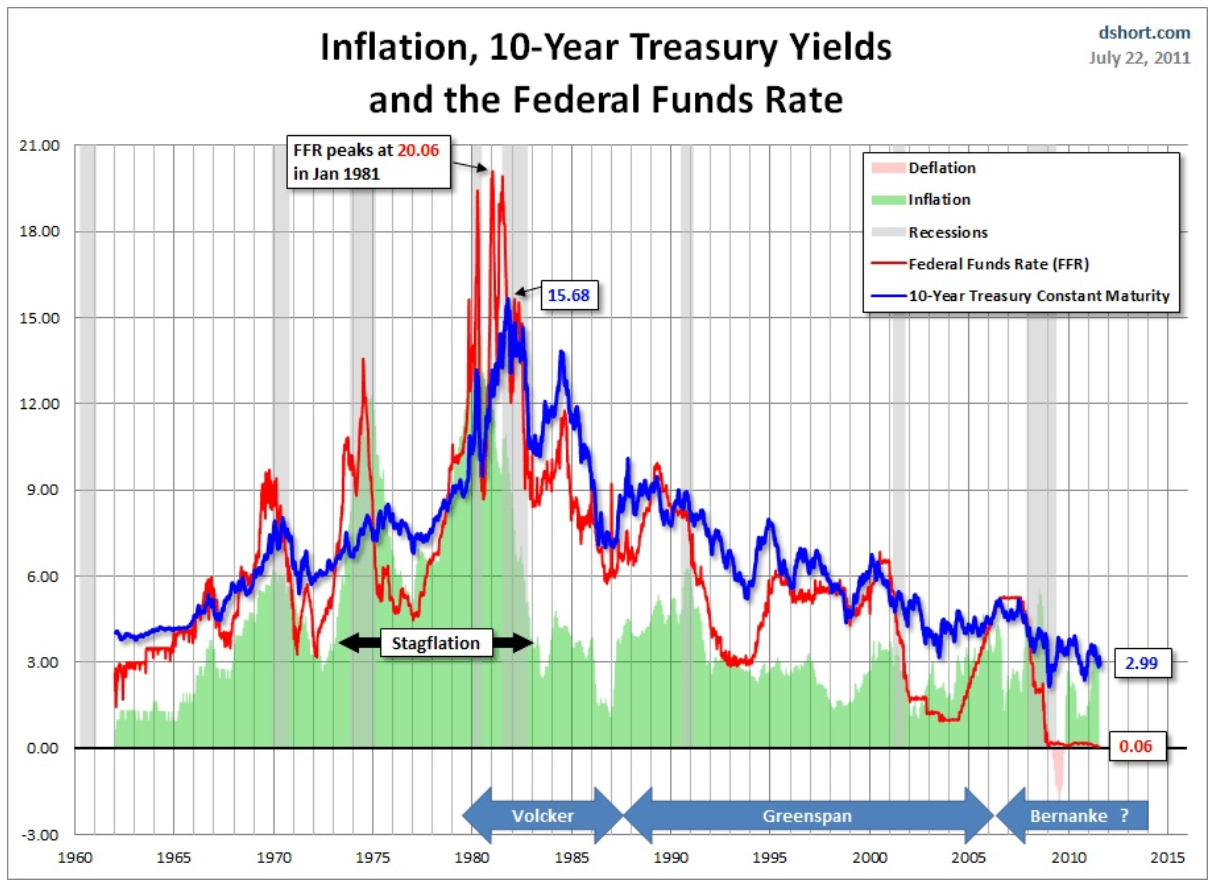
\includegraphics[width=1.1\textwidth]{images/ffr_inflation.png}}
    \caption{US inflation and target rate. }
    \label{fig:cpi_ffr}
\end{figure}

Trying to push rates negative might lead to mass withdrawals of money from banks. That would worsen a financial crisis, and ultimately impose a huge efficiency cost on the economy through the collapse of convenient electronic payments system. Worst of all, once we completed the awkward transition to a cash economy, interest rates would still effectively be stuck at zero — cash pays neither positive nor negative interest — so nothing would be accomplished.

% https://www.vox.com/cards/fed_vs_crisis/
Quantitative easing is often regarded as a form of "printing money" but the Fed doesn't literally print anything. Paper money is printed by the Bureau of Printing and Engraving so that people who want to take money out of their bank accounts can get their hands on cash. But most money is electronic. And, yes, quantitative easing involves the Fed making new money. It then uses that money to buy bonds, injecting extra money into the banking system. The money supply used to increase at a slow but steady pace, but during the 2007 financial crisis, it has instead shot up in several large irregular spurts associated with different rounds of QE. 

What makes it quantitative is that when the Fed does QE it specifies a dollar quantity of assets that it wants to buy. An alternative approach (call it qualitative easing, if you like) would be for the Fed to target a specific outcome it wants to see — conventional mortgage rates below X percent or whatever — and then commit to buying however many assets it takes to create that outcome.

Did all this QE create tons of inflation? No. Inflation was very low during Ben Bernanke's tenure in office. One reason for that is that even though lots of money has been created, much of it is simply parked at the Fed. Banks are required to hold reserves — that is, money that they don't lend out — as a regulatory matter. But lately they've been holding lots of extra reserve money. This stockpiling of excess reserves at the Fed may have happened in part because the Fed now pays interest on them to the banks. Paying interest on excess reserves could be a useful way for the Fed to in effect suck money out of the economy if it becomes worried about inflation in the future. No investment on Earth is safer for banks than parking money at the Fed, so the higher you make that interest rate the more money banks will park. Money that is parked is not being loaned out and spent. So by inducing banks to park their money, the Fed can put the breaks on the economy and stop inflation. 

Another line of criticism, associated with Paul Krugman's 1998 analysis of the Japanese economy, says that the real problem is something else. The Fed wants to reassure people that it has the ability to fight a potential future outbreak of inflation. But QE would be more potent if people were in fact afraid of a potential future outbreak of inflation. People worried that their money may lose value in the near future are more likely to run out and trade that cash for cars or refrigerators or houses and spur economic activity.